\chapter{Evaluation}
\label{cha:ergebnisse}

The robot is put into specific scenarios to trigger behavior responses from the behavior tree component. The scenario testing is done to evaluate the efficacy of the implemented behaviors in relation to the functional requirements listed in section \ref{sec:Requirements}.

The scenarios are executed in a simulated apartment environment as seen in figure \ref{fig:house_gazebo} and a simulated world with small round obstacles in an enclosed space as depicted in figure \ref{fig:world_gazebo}. The environments were mapped beforehand with the ROS2 "Slam Toolbox" package and provided by the Nav2 map server. 

\begin{figure}[ht]
	\centering
	\begin{subfigure}[b]{0.495\textwidth}
		\centering
		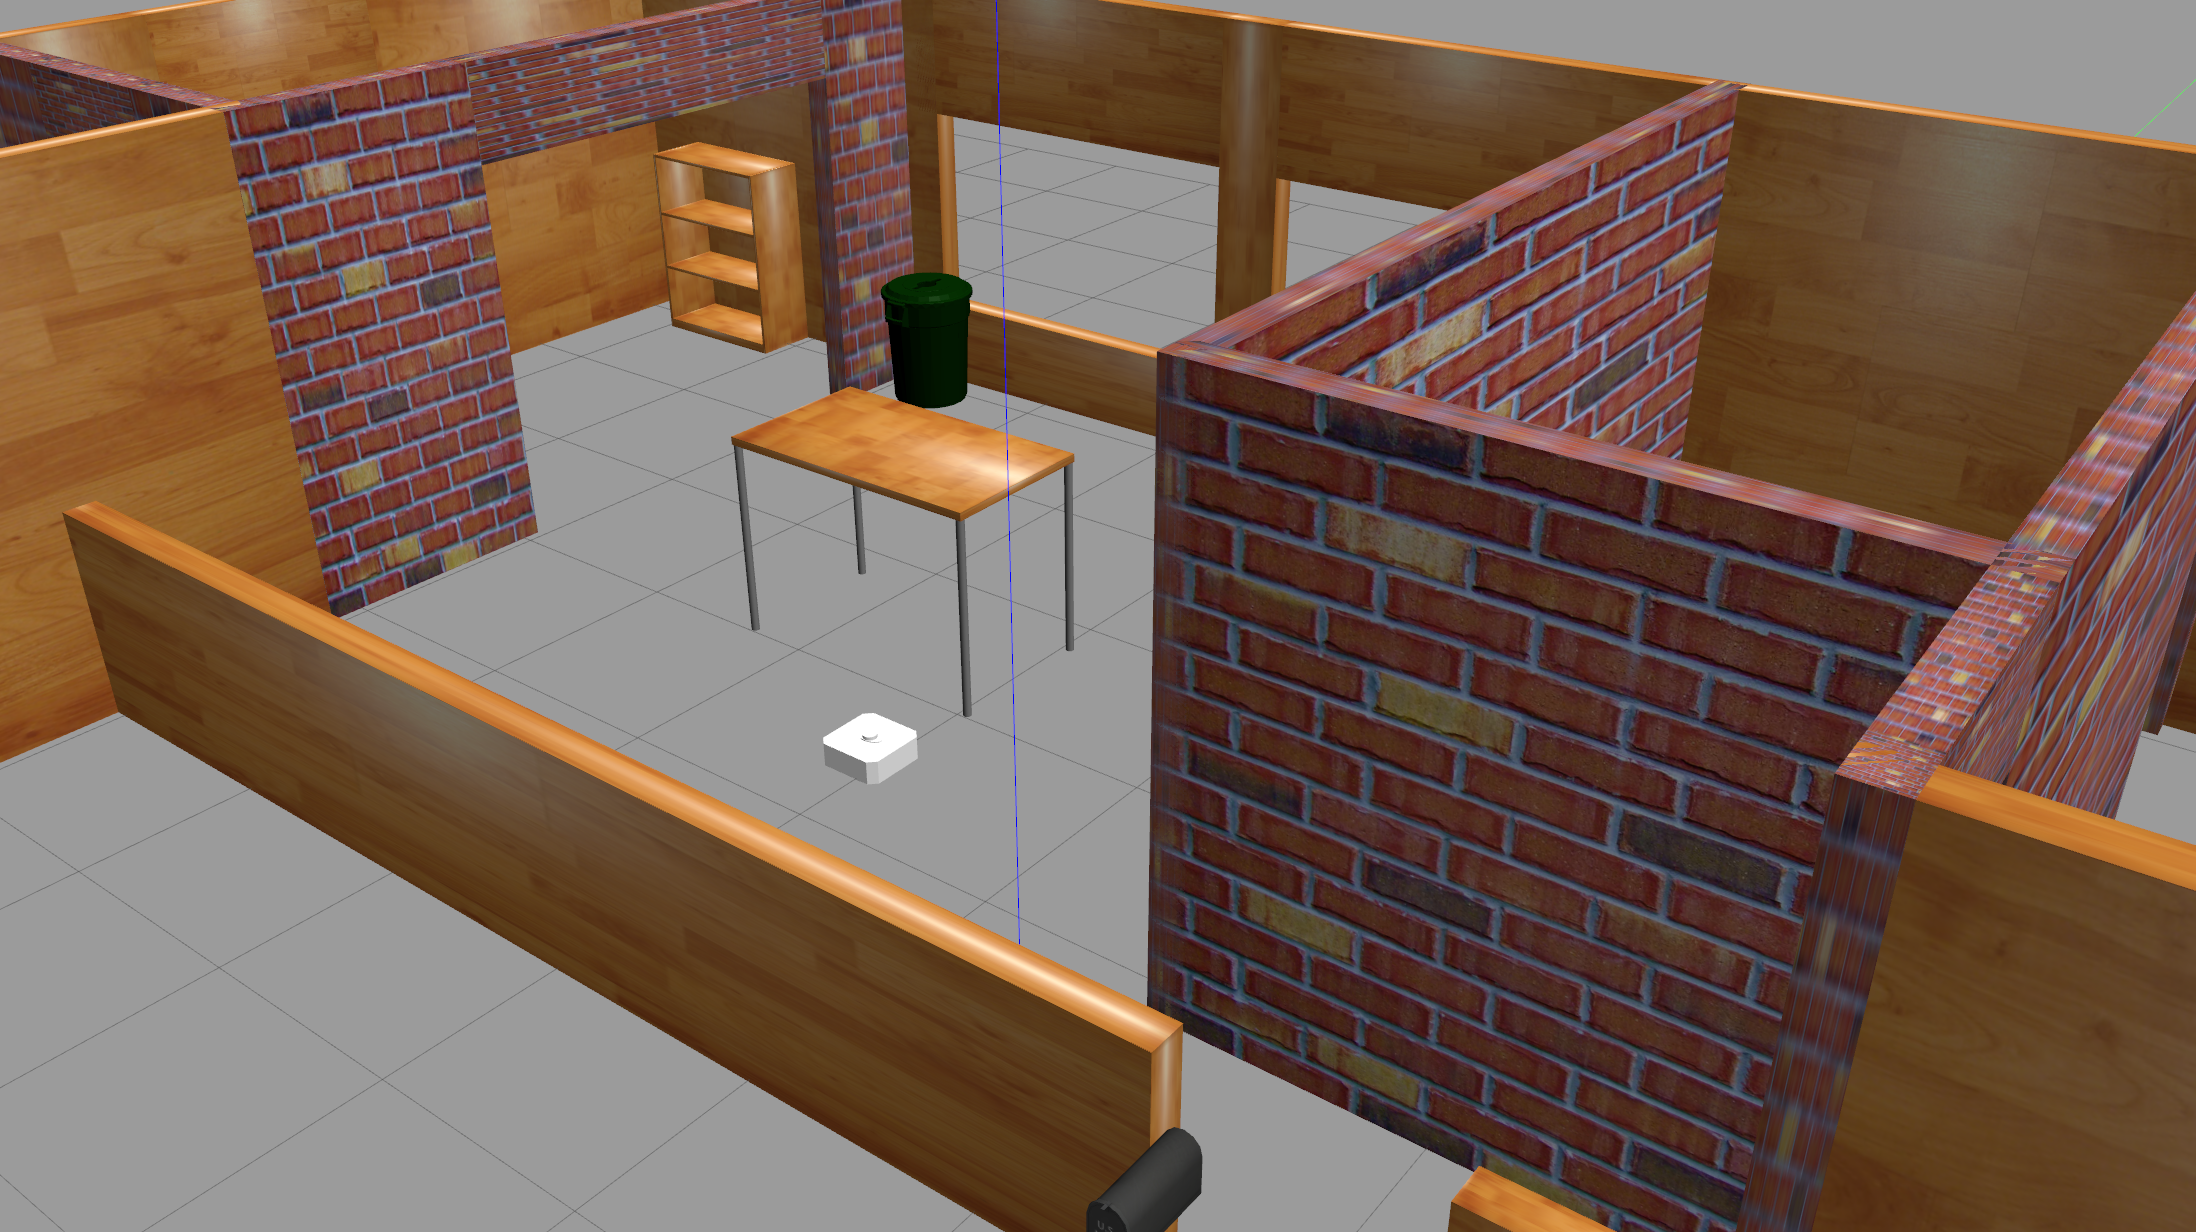
\includegraphics[width=\textwidth]{images/house_env.png}
		\caption{Apartment Environment in Gazebo}
		\label{fig:house_gazebo}
	\end{subfigure}
	\hfill
	\begin{subfigure}[b]{0.495\textwidth}
		\centering
		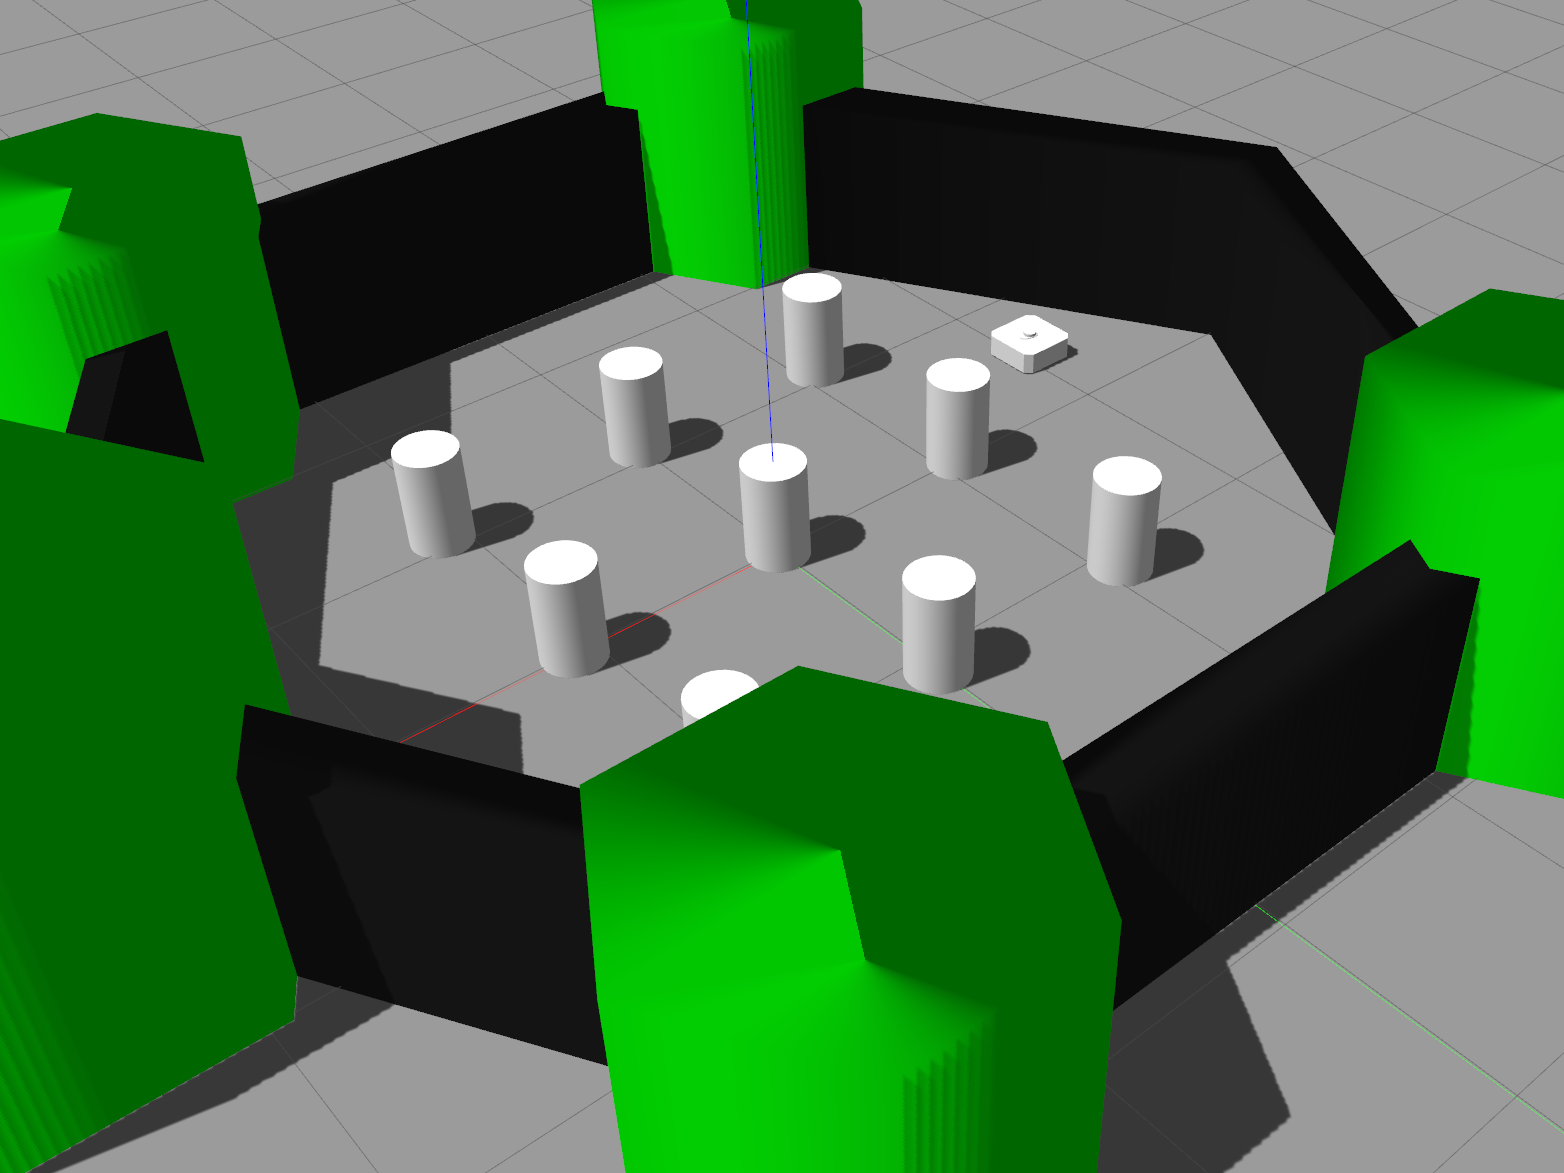
\includegraphics[width=\textwidth]{images/world_env.png}
		\caption{Enclosed Environment in Gazebo}
		\label{fig:world_gazebo}
	\end{subfigure}
	\caption{Gazebo World Environment}
	\label{fig:three graphs}
\end{figure}

The robot location and navigation goals are defined in another ROS node, which programmatically spawns the robot into the environment and sets the goal this way. This way, the same scenario can be run with and without behavior planning. To test the behavior of the sensor failure fallbacks, the respective sensor driver, mentioned in section \ref{subsec:gazebo_driver}, was shut down to emulate the sensor's failure. 

\section{Scenarios}

The scenarios are derived from the functional requirements and can be used to test multiple requirements as listed in the tables \ref{tab:sensor_scenarios} and \ref{tab:behavior_scenarios}. The acceptance criteria often contain multiple binary conditions that can only be met or failed. All acceptance criteria for a given scenario must be met for the test to be counted as a success. 

\begin{table}[ht]
	\centering
	\caption{Sensor Scenarios}
	\label{tab:sensor_scenarios}
	\renewcommand{\arraystretch}{1.5}
	\resizebox{0.99\textwidth}{!}{%
		\begin{tabular}{| m{0.11\textwidth}| m{0.1\textwidth} | m{0.183\textwidth}| m{0.3\textwidth} | m{0.3\textwidth}|} 
			\hline
			\textbf{Sensor Tested} & \textbf{Name} & \textbf{Requirements }& \textbf{Description} & \textbf{Success Criteria}\\ 
			\hline
			& Lidar$\_$1 & fn$\_$req1, fn$\_$req2, fn$\_$req3, fn$\_$req4, fn$\_$req5 & Robot is standing still, Lidar node crashes & Reset the system\\ 
			\cline{2-5}
			Lidar &Lidar$\_$2 & fn$\_$req1, fn$\_$req2, fn$\_$req3, fn$\_$req4, fn$\_$req5 & Navigating with 0.25 m/s straight towards goal (1m away) & Reset system, reach goal \\ 
			\cline{2-5}
			& Lidar$\_$3 & fn$\_$req1, fn$\_$req2, fn$\_$req3, fn$\_$req4, fn$\_$req5 & Navigating with 0.25 m/s and 0.5 rad/s towards goal (1m away) & Reset system, reach goal\\
			\hline
			& IMU$\_$1 & fn$\_$req1, fn$\_$req2, fn$\_$req3, fn$\_$req4, fn$\_$req5 & Robot is standing still, IMU node crashes & Reset system \\
			\cline{2-5}
			IMU &IMU$\_$2 & fn$\_$req1, fn$\_$req2, fn$\_$req3, fn$\_$req4, fn$\_$req5 & Navigating with 0.25 m/s straight towards goal (1m away) & Reset system, reach goal \\ 
			\cline{2-5}
			&IMU$\_$3 & fn$\_$req1, fn$\_$req2, fn$\_$req3, fn$\_$req4, fn$\_$req5 & Navigating with 0.25 m/s and 0.5 rad/s towards goal (1m away) & Reset system, reach goal\\
			\hline
			& Odom$\_$1 & fn$\_$req1, fn$\_$req2, fn$\_$req3, fn$\_$req4, fn$\_$req5 & Robot is standing still, Odom node crashes & Reset the system\\ 
			\cline{2-5}
			Odometry &Odom$\_$2 & fn$\_$req1, fn$\_$req2, fn$\_$req3, fn$\_$req4, fn$\_$req5 & Navigating with 0.25 m/s straight towards goal (1m away) & Reset system, reach goal \\ 
			\cline{2-5}
			&Odom$\_$3 & fn$\_$req1, fn$\_$req2, fn$\_$req3, fn$\_$req4, fn$\_$req5 & Navigating with 0.25 m/s and 0.5 rad/s towards goal (1m away) & Reset system, reach goal\\
			\hline
		\end{tabular}
	}
\end{table} 

\begin{table}[ht]
	\centering
	\caption{Behavior Scenarios}
	\label{tab:behavior_scenarios}
	\renewcommand{\arraystretch}{1.5}
	\resizebox{0.9\textwidth}{!}{%
		\begin{tabular}{| m{0.12\textwidth} | m{0.19\textwidth}| m{0.4\textwidth} | m{0.35\textwidth}|} 
			\hline
			\textbf{Name} & \textbf{Requirements} & \textbf{Description} & \textbf{Success Criteria}\\ 
			\hline	
			NoPath Found$\_$1 & fn$\_$req7 & Path to goal can not be calculated, robot is standing still & 
			Reset system, calculate path to goal, reach goal \\
			\hline
			NoPath Found$\_$2 & fn$\_$req7, fn$\_$req8 & Goal is unreachable, robot is standing still & Alternative goals, close to the original are tested to be reachable \\
			\hline
			Collision$\_$1 & fn$\_$req2, fn$\_$req4, fn$\_$req6 & Robot is standing still and a collision with the robot is caused & Robot can get out of collision state, navigation to goals still working \\
			\hline
			Collision$\_$2 & fn$\_$req2, fn$\_$req4, fn$\_$req6 & The robot is driving and collides with an undetected obstacle (0.25m/s) & 
			Robot can get out of collision state, navigation to goals still working, undetected obstacle gets added to map \\
			\hline
			Battery$\_$1 & fn$\_$req9 & The robot battery runs low & The robot will not drive to a goal that is outside of its reachable range \\
			\hline	
		\end{tabular}
	}
\end{table}	

The scenarios were conducted in different ways described in the following paragraphs.

For the lidar, IMU, and odometry scenarios, the sensor driver was shut down when reaching the desired speed listed in the scenario. The location and goal are given as described in the previous chapter. Each sensor was tested multiple times in three different driving situations. 

NoPathFound$\_$1 is a scenario in which the lifecycle state of the global planner gets transitioned into "inactive" and cannot execute the planning action anymore when triggered. The BT has to recover from the inability to plan in this scenario. NoPathFound$\_$2 simulates that the planner is active but fails to find a collision-free path to the desired goal. This scenario tests the ability to find alternative goals and navigate to a nearby goal. 

In the Collision$\_$1 scenario, an obstacle gets moved so close to the robot that a collision is registered. The forced collision tests the ability to maneuver out of a collision and resume navigation afterward. A new navigation goal is published after the behavior tree exits the Collision Fallback Routine. Collision$\_$2 tests the same behavior but during active navigation. A flat obstacle is spawned in the path of the robot. The obstacle is too low to be detected by the laserscanner, and a collision occurs. The robot must be able to recover from the crash and keep on navigating towards the goal with an updated global path. 

The Battery$\_$1 scenario tests if the robot tries to navigate toward a distant goal with a low battery charge. The simulated battery is emptied to a low level, and a new navigation goal is set. The test fails if the battery charge runs below zero percent during the navigation.

\section{Results}

The results in table \ref{tab:results} show an increase in the successful handling of the test scenarios for most test cases. The system supervision component is very reliable and enables the system to recover from an unexpected sensor failure. The more advanced behaviors can improve the autonomous handling of the scenarios. The Battery Scenario was successful every time it was induced. However, the path planning behavior for finding alternative goals was unsuccessful about 50 percent of the time. 

The collision behavior during driving worked well, and the map updates are an essential feature for the success of the test scenarios. Nevertheless, there is a lack of intelligence and autonomy when the robot stands still, and a collision is forced. The implemented behavior relies on the same mechanism as during the driving scenario. The missing differentiation led to a test case where the robot reversed into a wall because it was turned 90 degrees by the collision. Therefore, the test failed because a human operator would be needed to correct the robot's position. This lack of robustness was not apparent in the driving collision scenario because the robot's force was insufficient to cause a significant shift in orientation when colliding with obstacles. 

\begin{table}[ht]
	\centering
	\caption{Results}
	\label{tab:results}
	\renewcommand{\arraystretch}{1.5}
	\resizebox{0.9\textwidth}{!}{%
		\begin{tabular}{| m{0.11\textwidth} | m{0.11\textwidth}| m{0.235\textwidth} | m{0.19\textwidth}|} 
			\hline
			\multirow{2}{*}{\textbf{Name}} & \multirow{2}{0.11\textwidth}{\textbf{Number of Runs}} & \multicolumn{2}{|c|}{\textbf{Percentage Successful}} \\
			\cline{3-4}
			& & \textbf{Without Behavior Planning} & \textbf{With Behavior Planning} \\
			\hline
			Lidar$\_$1 & 5 & 0 & 100 \\ 
			\hline
			Lidar$\_$2 & 5 & 0 & 100 \\ 
			\hline
			Lidar$\_$3 & 5 & 0 & 100 \\ 
			\hline
			IMU$\_$1 & 5 & 0 & 100 \\ 
			\hline
			IMU$\_$2 & 5 & 0 & 100 \\ 
			\hline
			IMU$\_$3 & 5 & 0 & 100 \\ 
			\hline
			Odom$\_$1 & 5 & 0 & 100 \\ 
			\hline
			Odom$\_$2 & 5 & 0 & 100 \\ 
			\hline
			Odom$\_$3 & 5 & 0 & 100 \\ 
			\hline
			NoPath Found$\_$1 & 20 & 0 & 100 \\ 
			\hline
			NoPath Found$\_$2 & 20 & 0 & 55 \\ 
			\hline
			Collision$\_$1 & 20 & 0 & 95 \\ 
			\hline
			Collision$\_$2 & 20 & 0 & 100 \\ 
			\hline
			Battery$\_$1 & 10 & 0 & 100 \\ 
			\hline
		\end{tabular}
	}
\end{table} 

The results show that the functional requirements (as defined in \ref{sec:Requirements}) are met in almost all cases. Fn$\_$req1 to fn$\_$req5 are all completely fulfilled. Fn$\_$req6 is only partly fulfilled as the test showed potential shortcomings of the implemented collision behavior. Fn$\_$req7 satisfies the acceptance criteria, but fn$\_$req8 is only partly met by the implemented behavior to find alternative goals. Finally, the battery behavior meets all acceptance criteria, and fn$\_$req9 is fulfilled.

The architectural design choices meet all the non-functional requirements. Implementing the behavior planning and system supervision system eliminates a single point of failure for the system. Even when the Navigation2 system collapses, the robot can move to a degree and, more importantly, stop completely (compare table \ref{tab:nonfn_req}, non$\_$fn$\_$req). The behavior tree and algorithms implemented in the behavior tree are all deterministic (non$\_$fn$\_$req3). The robots' behavior goes beyond pure reactivity when navigating through environments, as the advanced behaviors use a dedicated planning phase before the actions are carried out (non$\_$fn$\_$req4). 

Finally, the system's performance when checking the conditions of the BT is below the desired threshold of 10ms, as the whole system runs in multiple threads, which allows the behavior tree to complete one complete execution cycle in about 5ms with the current system. (non$\_$fn$\_$req2). 